本章では、対象を如何にしてモデル化するかを、鉄道会社Aの特急券予約システムを例にして説明する。
これは、乗客として特急券予約システムを使う際に起きたトラブルの原因を追求するために作成したモデルである。

\section {特急券予約システムの例}
	\index{えくすぷれすよやくのれい@特急券予約システムの例}

\subsection{問題点の要約}
	\addcontentsline{toc}{section}{問題点の要約}
	\index{もんだいてんのようやく@問題点の要約}

問題の発端は、クレジットカード会社の都合で、
特急券予約システムに使用していたクレジットカードを変更せざるを得なくなり、
特急券予約システムの設定を変更しようとしたところから始まった。

\begin{enumerate}
\item 客(すなわち筆者)は、おサイフケータイ(鉄道会社B)で特急券予約システム(鉄道会社A)を使っていた。
\item 会社Cクレジットカードが廃止になり会社Dクレジットカードに変更して下さいとの連絡があった。
\item 鉄道会社Aサポートセンターに電話したところ、
	おサイフケータイの登録クレジットカードを変更すれば、2日後には特急券予約システムが使えますとのことだった。
\item おサイフケータイの設定でクレジットカードを変更し、2日後に使おうとしたが、特急券の予約ができなかった。
\item 予約できなかったので 鉄道会社Aサポートセンターに電話

	\begin{description}
	\item [客]「特急券を2枚予約しようとしたが、予約できなかったんですが?」
	\item [鉄道会社A]「カードを変更したら、新規に特急券予約システムを契約して下さい。」
	\item [客]「新規にすると会費がかかるのでは?」
	\item [鉄道会社A]「はい。」
	\item [客]「カード会社の都合で変更するのに、それはおかしいでしょう?」
	\item [鉄道会社A]「では、無料にします。」
	\end{description}

\item 特急券に引き換えできなかったので 鉄道会社Aサポートセンターに電話

	\begin{description}
	\item [客]「新しい予約はできたんですが、クレジットカード変更前に予約した特急券に引き換えようとしたらできないのですが?」
	\item [鉄道会社A]「予約会員証で引換できるようになったので、それで引き換えて下さい。
			暗証番号はクレジットカードのものを使って下さい。」
	\end{description}

\item T駅での問答

	\begin{description}
	\item [客]「会員証で特急券に引き換えできないのですが?」
	\item [鉄道会社A]「会員証で引き換えできないですねー。おかしいな。クレジットカードでやってみましょう。駄目ですねー。」
	\item [客]「古いクレジットカードでは駄目ですか?」
	\item [鉄道会社A]「あ、できましたね。はい、切符です。」
	\end{description}

\end{enumerate}

\subsection {モデル化対象用語の選択}
	\addcontentsline{toc}{section}{モデル化対象用語の選}
	\index{もでるかたいしょうようごのせんたく@モデル化対象用語の選択}


前節のやりとりは、電話でのやりとりをかなり(主として用語を中心として)整理したものである。
実際には、例えば、鉄道会社Aサポートセンターの担当者は「カード」という言い方をするのだが、
それがクレジットカードの場合と、予約会員証の場合と、
IC カードあるいは予約カードの場合があったので、
個々の用語の正確な名前と意味を調べるだけで
かなりの日数と時間を要した問答であった。

この問題で登場する用語は、インターネットなどで調べたところ以下に示すものががあった。

\begin{itemize}
\item 鉄道会社A、鉄道会社B
\item おサイフケータイ
\item 特急券予約システム
\item 予約会員証、ICカード、予約カード
\item クレジットカード
	\begin{itemize}
	\item 会社Cクレジットカード、会社Dクレジットカード
	\end{itemize} 
\item 特急券
\end{itemize} 

ICカードと予約カードは、結局、この問題とは直接は関係なかったので、
モデルを単純化するため対象としないことにした。

「鉄道会社B」をモデル化すると、さらに問題点が見つかるとは思ったが、
今回の「特急券に引き換えできない問題」の解決には直接関係ないと思ったので、
モデルを単純化するため対象としなかった。

このように、モデルを単純化し、一番問題となりそうなところからモデル化を始め、
検証して問題がないことを確認し、
必要があればモデルを拡張していくのがモデル化のコツである。

\subsection {モデル化する機能の範囲選択}
	\addcontentsline{toc}{section}{モデル化する機能の範囲選択}
	\index{もでるかするきのうのはんいせんたく@モデル化する機能の範囲選択}


「鉄道会社A」の「特急券予約システム」のうち、
今回の問題に直接関係する
以下の機能だけをVDM++\cite{Kyushu2016PP}で要求仕様としてモデル化し、
問題点を明確化することにした。
\footnote{仕様記述言語としてVDM++を採用したのは、
開発現場に導入するのが最も容易な形式仕様記述言語と判断したからである。
}

\begin{itemize}
\item 予約する
\item 特急券を得る
\item クレジットカードを切り替える
\end{itemize} 

したがって、モデル化する範囲に登場する主要な用語は以下だけである。
\begin{itemize}
\item おサイフケータイ
\item 特急券予約システム
\item 特急券予約
\item 予約会員証
\item クレジットカード
\item 特急券
\end{itemize} 

この用語と先程モデル化することにした機能を表す文(「予約する」、「特急券を得る」など)を併せて辞書とし、
要求辞書と呼ぶこともある。
	\index{ようきゅうじしょ@要求辞書}

\subsection {仕様記述フレームワークの設定}
	\addcontentsline{toc}{section}{仕様記述フレームワークの設定}
	\index{しようきじゅつふれーむわーくのせってい@仕様記述フレームワークの設定}
	\label{sec:specFM}

仕様を作成する際、仕様作成者各自が独自の形式で作成すると、
保守性や再利用性に悪影響が出る。
	\index{ほしゅせい@保守性}\index{さいりようせい@再利用性}

そこで、仕様を階層分けしてカプセル化し、
	\index{かぷせるか@カプセル化}
各階層で充足すべき記述領域を明確化して、保守性と再利用性の向上を図った。

このような仕様記述フレームワークを作っておくと、
各階層毎の記述に必要なVDM++言語の知識も局所化でき、
全員がVDM++に精通していなくても、仕様記述が可能になることが、
経験上分かっている。

本モデルの記述に際して使用する仕様記述フレームワークの階層は、表\ref{SpecLevel1}のようになる。

\begin{table}[h]
	\caption[仕様の階層(特急券予約システム)]{仕様の階層(特急券予約システム)}
	\index{しようのかいそうとっきゅうけんよやくしすてむ@仕様の階層(特急券予約システム)}
	\label{SpecLevel1}
	\begin{center}
		\setlength{\tabcolsep}{3pt}
		\begin{tabular}{|l|l|l|l|} \hline
			仕様記述の階層 & 充足する記述領域 & 備考 & 必要なVDM技量  \\ \hline\hline
			テスト & 回帰テスト & & 初級 \\ \hline
			業務論理 & 業務アプリケーション &  構造化日本語仕様 & 初級\\ \hline
			要求辞書 & 業務知識兼用語辞書 & ドメイン・オブジェクトも含まれる & 中級 \\ \hline
			ユーティリティ & 共通機能 & & 上級〜中級 \\ \hline
		\end{tabular}
	\end{center}
\end{table}

表\ref{SpecLevel1}で、業務論理階層の記述は、
業務アプリケーションを記述する日本語識別子を使った構造化日本語仕様と見なすこともできる。

日本語で擬似コードを使った仕様を書くことがあるが、
この場合は逆に、厳密で明確な文法を持ったVDM++の仕様を日本語による擬似コードのように読めるよう工夫することで、
読みやすさと厳密な記述による品質向上の両方を目指そうという訳である。


\subsection {VDM++モデル例}	
	\addcontentsline{toc}{section}{VDM++モデル例}
	\index{VDM++モデルれい@VDM++モデル例}
	\label{VDMModelExpressReservation}

以下に、特急券予約システムをVDM++で記述したモデルを示す。
	\index{とっきゅうけんよやくしすてむをVDM++できじゅつしたもでる@特急券予約システムをVDM++で記述したモデル}

このモデルは、要求仕様記述レベルであるが、
アプリケーションレベルのエラー処理は記述せず、
不変条件と事前条件および事後条件の記述を行う。
すなわち、要求仕様記述・分析工程で最初に記述し検証する、
最も抽象的なモデルである。
	\index{ちゅうしょうてきなもでる@抽象的なモデル}

要求仕様記述・分析工程の最後では、
アプリケーションレベルのエラー処理をすべて記述する、
詳細な要求仕様を記述するが、
	\index{しょうさいなようきゅうしよう@詳細な要求仕様}
通常、その規模は最初の抽象的な要求仕様より10倍ほどになるので、
本ブックレットでは紹介できなかった。

静的検証と動的検証の両方を使って正当性検証と妥当性確認を行う。
動的検証は、仕様アニメーション、すなわち仕様実行によって行う。

特急券予約システムの、主要なクラスを記述したクラス図は図\ref{fig:ExpressReservationClassDiagram}のようになった。
このクラス図は、最初からこのような形をしていたわけではなく、
VDM++でモデル化をしつつ、検証しながら、徐々に整理してこのような形となった。
\footnote{
このクラス図は、VDMToolsから生成し、astah professionalによって整形したものである。
}

\begin{figure}[h]
	\centering
	{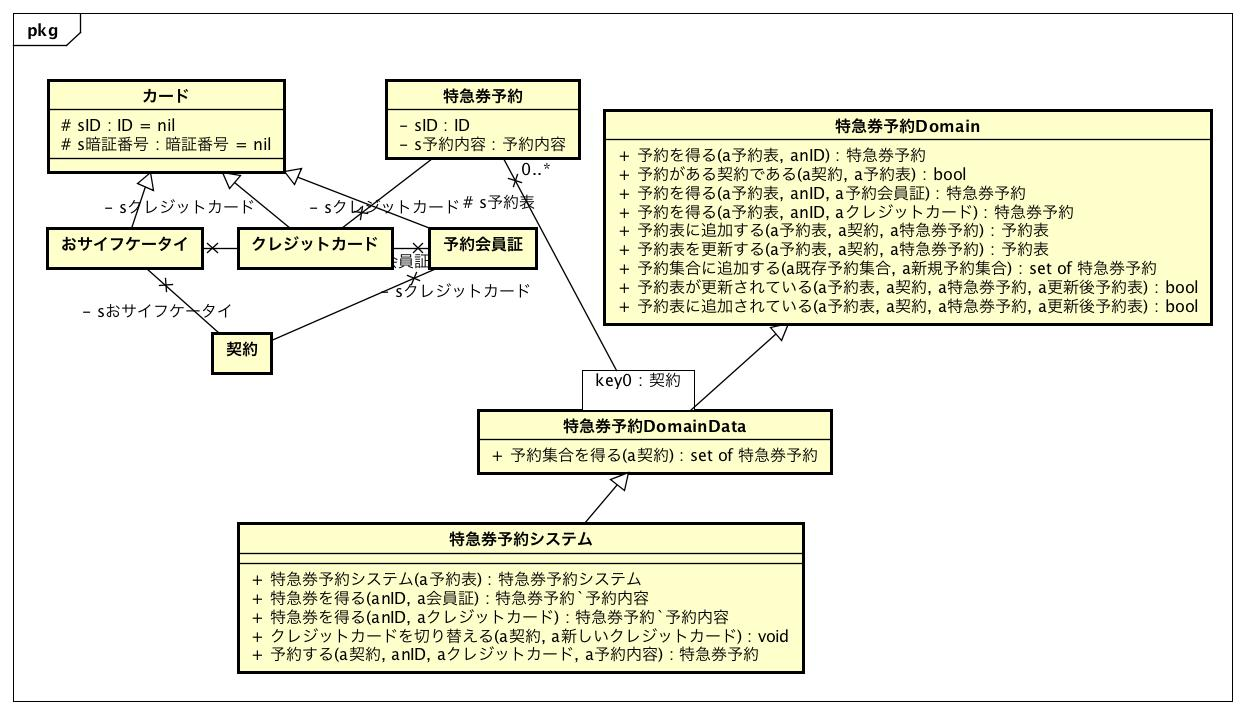
\includegraphics[width=55zw, keepaspectratio]{./ExpressReservation/image/ClassDiagram.jpg}}
	\caption{クラス図(特急券予約システム)}
	\label{fig:ExpressReservationClassDiagram}
	\index{くらすすとっきゅうけんよやくしすてむ@クラス図(特急券予約システム)}
\end{figure}

各クラスと、仕様階層の対応は、表\ref{SpecLevel2}のようになる。

\begin{table}[h]
	\caption[特急券予約システムの仕様の階層]{特急券予約システムの仕様の階層}
	\index{えくすぷれすよやくのしようのかいそう@特急券予約システムの仕様の階層}
	\label{SpecLevel2}
	\begin{center}
		\setlength{\tabcolsep}{3pt}
		\begin{tabular}{|c|l|} \hline
			階層 & クラス   \\ \hline\hline
			テスト & TestApp \\ \cline {2-2}
			  & 回帰テストケースクラス(TestCaseT0001など) \\ \hline
			業務論理 & 特急券予約システム \\ \hline
			要求辞書 & 特急券予約システムDomain   \\ \cline {2-2}
			  & 特急券予約システムDomainData \\ \cline {2-2}
			  & 契約   \\ \cline {2-2}
			  & 特急券予約システム  \\ \cline {2-2}
			  & クレジットカード  \\ \cline {2-2}
			  & 予約会員証  \\ \cline {2-2}
			  & おサイフケータイ \\ \hline
			ユーティリティ & 回帰テストユーティリティなど \\ \hline
		\end{tabular}
	\end{center}
\end{table}

